\documentclass[../main.tex]{subfiles}

\begin{document}

Unter einer General Purpose x86 CPU werden Prozessoren verstanden, die den Befehlssatz und die Architektur x86 verwenden. Diese Architektur wird von den beiden großen CPU Herstellern Intel und AMD verwendet und befindet sich somit in nahezu allen PCs und Laptops. 

Heutige CPUs dieser Hersteller verstehen wesentlich mehr Instruktionen als der klassische x86-Befehlssatz. Somit bestehen heute einige Möglichkeiten, den Programmcode für diese Architektur zu optimieren. Eine dieser Optimierungsmöglichkeiten ist die Verwendung von SIMD-Instruktionen (Single Instruction, Multiple Data). Damit können mehrere Rechenoperationen gleichzeitig in speziellen Registern ausgeführt werden.
Eine weitere Optimierungsmöglichkeit ergibt sich aus der Tatsache,  dass CPUs heute aus mehrere CPU Kernen bestehen. Dadurch können Instruktionen gleichzeitig auf mehreren Kernen parallel ausgeführt werden.

Zur Entwicklung des Programms wurde Eclipse CDT verwendet und als Compiler gcc, ein weit verbreiteter Compiler mit einer großen Open Source Comunity. Dieser kann mit sehr vielen Flags aufgerufen werden, um den Compiliervorgang optimal einzustellen.

Ein optimiertes Neuronales Netzwerk auf der General Purpose x86 CPU wurde im Rahmen dieser Arbeit nicht erfolgreich Implementiert. Alle Funktionen eines Neuronalen Netzwerkes wurde zwar implementiert und bei einer geringen Menge von Trainingsdaten werden diese nach vielen Iterationen auch richtig erkannt. Das Erkennen von neuen Daten ist jedoch selbst nach einer langen Zeitspanne zum Trainieren nicht möglich und die Iterationen zum Trainieren des Netzwerkes sind um ein vielfaches höher als von anderen Implementierungen des selben Netzes. Dabei muss es sich um einen Fehler in der Implementierung handeln, der bis zum Ende der Zeit für die Studienarbeit nicht gefunden werden konnte.
Die Suche nach dem Fehler war sehr schwer, da alle trainierten Werte des Neuronalen Netzwerk stimmen könnten und anhand der Werte nicht auf den Fehler geschlossen werden kann, was im Grundprinzip eines neuronalen Netzwerkes liegt. Die Zahlenwerte sind für einen Menschen nichtssagend und könnten alle plausibel sein.
Durch die langwierige Fehlersuche wurde der Code nicht ausreichend für die Zielhardware optimiert, sodass der Code nicht performant läuft.

\section{OpenMP (Open Multi Procesing)}

Aktuelle CPUs, ob im Arbeitsrechner, Laptop, Tablet oder Smartphone, besitzen inzwischen mehrere CPU-Kerne. Dies liegt daran, dass in den letzten Jahren der Mehrgewinn neuer CPUs nicht mehr durch eine erhöhten Taktfrequenz, wie in den Jahrzehnten zuvor, sondern durch eine parallele Verarbeitung von Daten erzielt wurde. Um das volle Potenzial dieser CPUs auszunutzen ist es zwingend notwendig, Programme zu parallelisieren, sodass Programmabschnitte auf mehreren Kernen gleichzeitig ausgeführt werden können.
„Unter der Parallelisierung eines Programms versteht man, dass mehrere Teile einer Aufgabe gleichzeitig nebeneinander ausgeführt werden, um so die Gesamtaufgabe schneller als bei strikt serieller Verarbeitung zu beenden." \cite{articleOpenMP}

Mit der Programmierschnittstelle OpenMP ist es relativ einfach Programme, mithilfe von Direktiven die in den Programmcode eingefügt werden, parallel ablaufen zu lassen. OpenMP ist hierbei für die Programmiersprachen C, C++ und Fortran verfügbar.

\subsection{Prozesse und Threads}

"Als Prozess bezeichnet man ein Programm, das gerade vom Betriebssystem ausgeführt wird." \cite{articleOpenMP} Ein Prozess wird auch als aktive Instanz eines Programmcodes bezeichnet. Systeme, die mehrere Prozesse scheinbar gleichzeitig ausführen können, werden als Multitasking Systemen bezeichnet. Eine tatsächliche parallele Ausführung ist jedoch oft nicht möglich, stattdessen werden verschiedene Prozesse nacheinander in kurzen Intervallen ausgeführt. Der Prozess Scheduler bestimmt hierbei, welcher Prozess wann ausgeführt wird. \par
Es gibt verschiedene Scheduling-Strategienum um zu bestimmen, wie lange und wann ein Prozess auf der CPU ausgeführt wird. Zu den bekanntesten gehört "First-Come First-Serve", "Shortest Job First" und Round Robin. Bei "First-Come First-Serve" werden alle Prozesse hintereinander in eine Warteschlange gestellt und müssen darauf warten, bis alle vorherigen Prozesse ausgeführt wurden.  Bei der Strategie "Shortest Job First" werden Prozesse, die nur kurze Ausführungszeiten benötigen, zuerst ausgeführt. Dies führt zu einer verringerten durchschnittlichen Wartezeit, Prozesse die eine lange Ausführungszeit haben brauchen aber sehr lange um ausgeführt zu werden.
Beim "Round Robin" Verfahren werden lange Prozesse in mehrere Teilstücke aufgeteilt. Nacheinander werden von jedem Prozess ein Teilstück abgearbeitet. Dadurch werden Prozesse, die viel Ausführungszeit benötigen, schneller abgearbeitet als bei "Shortest Job First" und Prozesse mit geringer Ausführungsdauer müssen nicht so lange warten wie bei "First-Come First-Serve". 
Neue Betriebssysteme arbeiten mit komplexeren Scheduling-Strategien, in denen Prozesse unterschiedliche Prioritäten bekommen und sich unterschiedlich "nett" gegenüber dem Prozessor verhalten können. \cite{scriptProzessScheduling}

Ein Prozess besteht aus folgenden Komponenten:
\begin{itemize}
	\item einer eindeutigen Prozess-ID
	\item dem auszuführenden Programmcode mit aktuellen Wert des Programmschrittzählers
	\item den aktuellen CPU-Registerwerten
	\item dem Stack zur Ausführung des Programms
	\item einen Datenbereich mit den globale Variablen
	\item dem Heap mit den dynamisch angelegte Variablen
\end{itemize} \cite{articleOpenMP}

Wird der Prozess, der zurzeit bearbeitet wird, gewechselt, müssen alle zu diesem Prozess gehörenden Daten gesichert werden. Der Bereich, in dem die Daten der einzelnen Prozesse liegen, wird Prozesskontrollblock genannt.

"In modernen Betriebssystemen kann ein Prozess über mehrere Ausführungsstränge oder Threads verfügen. Ein Thread kann als „Light-Version“ eines Prozesses betrachtet werden." \cite{articleOpenMP}
Mehrere Thread können sich einen Datenspeicherbereich, den Heap und andere Elemente eines Prozesses teilen. Dadurch kann der Wechsel zwischen Threads viel schneller erfolgen, als der Wechsel zwischen Prozessen. Des weiteren können Threads, durch den gemeinsamen Speicherbereich, auch tatsächlich parallel, auf mehreren CPU Kernen, bearbeitet werden.
OpenMP ermöglicht die einfache Nutzung dieser Technik. Es muss sich mit OpenMP nicht um die richtige Initialisierung oder das Erstellen und Beenden von Threads Gedanken gemacht werden. Stattdessen werden im Programmcode durch Compilerdirektiven einfach zu verstehende Anweisungen gegeben und dem Rest OpemMP überlassen. \cite{articleOpenMP}

\subsection{Programmiermodell}

Die nebenläufige Abarbeitung von Programmteilen wird bei OpenMP durch das Fork-Join-Prinzip erzielt. Dabei erfolgt an einer bestimmten Stelle im Programmcode ein sogenannter Fork. An dieser Punkt erzeugt der Thread, der den vorherigen Programmcode ausgeführt hat, neue Threads, die den danach folgenden Code parallel ausführen. Der Thread, der die anderen Threads erzeugt hat, wird Master-Thread genannt. Am Ende des parallelen Bereichs geschieht ein Join. Bei einem Join werden alle Treads synchronisiert und beendet. Lediglich der Master-Thread bleibt erhalten und führt das weitere Programm seriell aus. Zum Ausführen des Joins, müssen alle Threads die Ausführung des Codes beendet haben.

OpenMP erlaubt es, einen Fork auch innerhalb eines parallelen Programmabschnittes zu tätigen. Der außerhalb liegende Join muss dann auf alle innere Joins warten, also bis alle innerhalb des parallelen Codes erzeugten Threads beendet wurden.

\subsection{OpenMP-Direktiven}

Im folgenden Abschnitt sind alle Programmbeispiele in C- oder C++-Syntax gehalten. Die selben Anweisungen sind auch in Fortran möglich, können sich jedoch in der Erscheinungsweise unterscheiden.

Um Funktionen der Laufzeitbibliothek zu verwenden, muss die Datei \texttt{omp.h} in das C++-Projekt includiert werden. Es ist auch möglich, Anweisungen von OpenMP ohne die Verwendung der Laufzeitbibliothek zu verwenden, jedoch nicht mit jedem Compiler. Es wird deswegen empfohlen, die Bibliothek immer in das Projekt einzubinden \cite{articleOpenMP}. Um dem Conpiler gcc anzuweisen, dass er den Code unter Berücksichtigung von OpenMP übersetzen soll, muss das Compilerflag \texttt{-fopenmp} beim compilieren angegeben werden. \par
Mit der Compiler-Direktiven \texttt{\#pragma\ omp\ parallel} kann ein Codeabschnitt parallel abgearbeitet werden. Der Codeabschnitt wird von geschwungenen Klammern umschlossen. Die Klammer muss hierbei in der sich unterhalb der Direktiven befindenden Zeile eingefügt werden. Eine Geschwungene Klammer in der selben Zeile, hinter der Compilerdirektive, ist nicht zulässig \cite{articleOpenMP}. Von Compilern, die OpenMP nicht unterstützen, wird die Zeile mit der Direktive ignoriert. Da von Compilern, die OpenMP nicht unterstützen, die Bibliothek \texttt{omp.h} nicht gefunden wird, führt dies an der Stelle im Quellcode zu einem Fehler. Mit dem unterhalb stehenden Code wird die Bibliothek nur dann geladen, wenn der Compiler OpenMP unterstützt. Somit kann der gleiche Programmcode als paralleles oder als serielles Programm compiliert werden.
\begin{lstlisting}[language=c++, caption=Includieren der Bibliothek omp.h, captionpos=b, label=listing:include_omp, frame=single, linewidth=\textwidth, breaklines=true]
#ifdef _OPENMP
#include <omp.h>
#endif
\end{lstlisting}
Alle Direktiven in OpenMP sind nach diesem Muster aufgebaut \texttt{\#pragma\ omp\ <Direktive>\ [Klausel\ [[,]\ Klausel\ ]\ ...]}

\subsection{Variablen}

Variablen können entweder privat oder gemeinsam innerhalb eines parallelen Abschnitts deklariert werden. \par Eine gemeinsame Variable kann von verschiedenen Threads genutzt werden, während eine private Variable für jeden Thread einen anderen Wert annehmen kann. Gemeinsame Variablen werden mit dem Parameter \texttt{shared(Liste\_der\_Variablen)} deklariert. In der Liste werden alle Variablen hineingeschrieben, die gemeinsam genutzt werden sollen. Die Variablen sind mit dem Wert initialisiert, die sie vor dem Fork hatten. \par Private Variablen können hingegen mit \texttt{private(Liste\_der\_Variablen)} deklariert werden.  Anders als die Gemeinsamen Variablen sind diese anfangs nicht initialisiert, mit Ausnahme von Objekten die einen Konstruktur besitzen und Indexvariablen von Schleifen. Alle anderen privaten Variablen müssen im parallelen Code initialisiert werden. \par
Soll der Wert, den die Variable vor Beginn der parallelen Ausführung hatte, im parallelen Abschnitt verwendet werden, muss dafür der zusätzliche Parameter \texttt{firstprivate(Liste\_der\_Variablen)} verwendet werden. Der letzte Wert vor Ausführung des Forks wird dann als Anfangswert der privaten Kopien verwendet. \par Soll der Wert der Variable nach dem Join im weiteren Programmablauf verwendet werden, muss hierfür der zusätzliche Parameter \texttt{lastprivate(Liste\_der\_Variablen)} verwendet werden. Dabei wird der Wert, den die Variable bei serieller Ausführung am Ende des Abschnitts hätte als Wert für die Variable nach dem Join verwendet. Es ist auch möglich, dass eine Variable in beiden dieser zusätzlichen Parameter enthalten ist.

Eine weitere Möglichkeit der Deklaration von Variablen ergibt sich durch die Reduktionsvariablen. Diese funktionieren wie private Variablen, bis zum Zeitpunkt des Joins. Bei Reduktionsvariablen werden alle Werte der privaten Variablen durch eine Operation zusammengefasst. Bei dieser Operation kann es sich um die Addition, Subtraktion, Multiplikation, XOR, binäre und logische Und-Verknüpfung oder binäre und logische Oder-Verknüpfung handeln. Der Parameter für Reduktionsvariablen lautet \texttt{reduction( op:Liste\_der\_Variablen)}.

„Wird eine Variable in keiner der Deklarationen erwähnt, wird sie standardmäßig als gemeinsame Variable deklariert. Eine Ausnahme hiervon bildet die bei der Aufteilung einer Schleife auf mehrere Threads erzeugte Index-Variable der Schleife, die standardmäßig als private Variable deklariert wird. Soll ein explizites Deklarieren jeder im parallelen Bereich verwendeten Variable erzwungen werden, so wird der Direktive zusätzlich der Parameter default(none) hinzugefügt.“ (Uni München)
Das Default-Verhalten lässt sich jedoch auch ändern, dafür gibt es die Datenzugriffsklausel \texttt{default(zugriffsverhalten)}. Hier kann auch der Wert \texttt{none} angegeben werden. Dann gibt es für jede Variable, für die nicht explizit das Zugriffsverhalten angegeben wurde, beim compilieren einen Fehler. Dies kann für Testzwecke in den Code eingebaut werden, um sich für jede Variable explizit Gedanken zu machen.
Variablen können nur in einer Datenzugriffsklausel vorkommen, also nicht gleichzeitig privat und shared deklariert sein.

\subsection{Parallele Abarbeitung}

Parallele Abschnitte des Programms beginnen immer mit der Direktiven \texttt{\#pragma omp parallel}. Der sich innerhalb der geschwungenen Klammern befindende Code wird dann vom Compiler, wenn er OpenMP unterstützt, als parallelen Code übersetzt. Der Auszuführende Code ist hierbei, ohne Angabe weiterer Direktiven, in jedem Thread derselbe. 

Die Nummer des Threads, der den Aktuellen Code ausführt, kann mit \linebreak \texttt{omp\_get\_thread\_num} ermittelt werden. Die Gesamtanzahl der Threads wird bei Aufruf von \texttt{omp\_get\_num\_threads} zurückgegeben.

Die bei der Implementierung des Neuronalen Netzwerkes am meisten verwendete Direktive von OpenMP ist \texttt{\#pragma omp for [Parameter]}. Diese muss vor eine For-Schleife innerhalb eines parallelen Abschnittes gesetzt werden. Die For-Schleife wird dann parallel abgearbeitet, wobei jeder Thread nur eine Teilmenge der Iterationen abarbeitet. Eine Bedingung zur Verwendung dieser Direktiven ist, dass die Schleife in kanonischer Form vorliegt. Für die kanonische Form muss die Anzahl der Durchläufe dafür schon vor Beginn des ersten Durchlaufs berechenbar sein. Außerdem darf kein Ergebnis eines Schleifendurchlaufs zur Berechnung eines Ergebnis in einem anderen Durchlauf benötigt werden. Die Operation zum Vergleichen der Zählvariable darf nur \texttt{>, >=, <} oder texttt{<=} annehmen und die Zählvariable darf nicht durch eine Multiplikation oder Division erhöht oder verringert werden

Falls sich in einem parallelen Abschnitt nur eine for-Schleife befindet, kann die Direktive zusammengefasst werden. Die Anweisung heißt dann \texttt{\#pragma\ omp\ parallel\ for}. Die geschwungenen Klammern um den parallelen Code entfallen hierbei, da die for-Schleife bereits durch geschwungene Klammern ein Codesegment umschließt. Die zwei unten stehenden Codes bewirkt somit dasselbe.

\begin{lstlisting}[language=c++, caption=For innerhalb eines parallelen Abschnitts, captionpos=b, label=listing:for_in_parallel, frame=single, linewidth=\textwidth, breaklines=true]
#pragma omp parallel
{
   #pragma omp for
   for(...){
   }
}
\end{lstlisting}


\begin{lstlisting}[language=c++, caption=Kurzschreibweise einer parallelen For-Schleife, captionpos=b, label=listing:parallel_for, frame=single, linewidth=\textwidth, breaklines=true]
#pragma omp parallel for
for(...){
}
\end{lstlisting}

Als Parameter für die Direktive \texttt{\#pragma omp for} kann die Schedule-Strategie angegeben werden. Für eine statische Strategie, bei der eine bestimmte Anzahl an Interationen statisch auf die Threads verteilt werden, gibt es den Parameter \texttt{schedule(static, [Blockgröße])}. Die Blockgröße kann optional angegeben werden. Wird sie nicht angegeben, werden alle Iterationen durch die Anzahl der Threads geteilt und diese Anzahl verwendet. Wird die Blockgröße angegeben, darf diese nicht so klein sein, dass nicht alle Iterationen der Schleife von den Threads abgearbeitet werden. Der letzte Thread darf, wenn die Iterationsanzahl nicht gleichmäßig aufgeteilt werden kann, weniger Iterationen ausführen. Wird die Blockgröße sehr groß gewählt, sind unter Umständen nicht alle Threads mit der Abarbeitung der Schleife beschäftigt.
Bei einer dynamischen Verteilung muss der Parameter \texttt{schedule(dynamic, [Blockgröße])} angegeben werden. Hierbei wird die Blockgröße kleiner gewählt und die Threads arbeiten mehrere Blöcke mit Iterationen nacheinander ab. Sollten einige Iterationen länger dauern als andere, bekommen die Threads somit weniger Blöcke zur Abarbeitung. Die verhindert, dass gegen Ende der Abarbeitung ein einziger Thread noch rechnen muss, währenddessen alle anderen Threads schon lange fertig sind.
Die letzte Schedule-Strategie in OpenMP kann mit der Direktiven \texttt{schedule(guided, [Blockgröße])} verwendet werden. Dies ist eine spezielle Form der dynamischen Strategie. Hierbei werden die Blöcke zur Abarbeitung exponentiell immer kleiner. Iterationsblöcke, die schneller fertig werden, bekommen deshalb einen größeren zweiten Block als Iterationen, die später ihren ersten Block abgearbeitet haben. Die Unterschiede zwischen den Bearbeitungszeiten der Iterationsblöcke soll dadurch verringert werden.

Dynamische Ablaufpläne haben den Vorteil, dass die Threads auch bei unterschiedlicher Abarbeitungsdauer der Iterationen ungefähr gleichzeitig fertig werden mit ihren Berechnungen. Dennoch hat die statische Strategie ihre Daseinsberechtigung. Durch die dynamische Verwaltung entsteht ein großer Verwaltungsaufwand, da die Threads synchronisiert werden müssen und neue Iterationen den Threads zugewiesen werden müssen. Bei der statischen Strategie hingegen wird dieser Aufwand nicht benötigt. Besonders, wenn sich die Abarbeitungszeiten der Iterationen nicht verändert, kann es deswegen sinnvoll sein, auf die dynamische Strategie zu verzichten und stattdessen die statische Strategie zu verwenden.

An Ende der Schleife wird normalerweise darauf gewartet, bis alle Threads beendet werden können. Soll dies nicht geschehen, kann der Parameter \texttt{nowait} angegeben werden. Dann führen die Threads den folgendes Code aus, anstelle darauf zu warten bis alle Threads mit der Abarbeitung der parallelisierten Schleife fertig sind.

Ein weiterer Parameter zur Parallelisierung einer For-Schleife ist \texttt{ordered}. Dabei werden die Iterationen in der Reihenfolge ausgeführt, wie Sie bei paralleler Ausführung ausgeführt würden. Bei diesem Parameter kann noch ein Block mit dem Direktiv \texttt{\#pragma omp ordered} unterhalb der For-Schleife stehen. Dieser wird dann auch in der Reihenfolge ausgeführt, als wäre es serieller Code.

Weitere Funktionen zur Parallelisierung mit Hilfe von OpenMP wurden für diese Arbeit nicht verwendet und werden deswegen im Folgenden nur kurz erwähnt.
Für verschiedenen Bereiche, die unabhängig voneinander sind und parallel ausgeführt werden sollen, kann \texttt{\#pragma imp parallel section [Parameter]} verwendet werden.
Für kritische Abschnitte gibt es \texttt{\#pragma omp critical [(name)]} und eine Barriere kann mit \texttt{\#pragma omp barrier} erzeugt werden.

\section{Verwendung von SIMD auf x86 Architektur}

Eine weitere Optimierung ergibt sich durch die Verwendung von SIMD (Single Instruction, Multiple Data) Operationen.  Neue CPUs von Intel und AMD besitzen spezielle Register, auf die SIMD Operationen angewandt werden können. 
Die ersten SIMD Operationen auf der x86-Architektur von Intel wurden 1997 durch die Veröffentlichung von Prozessoren mit der Multi Media Extension (MMX) eingefügt. Die MMX beinhaltete 8 Register mit einer Größe von 64 Bit, die packed Integer Werte annehmen kann. Die Register hießen \texttt{mm0} bis \texttt{mm7}.
Von packed ist die Rede, wenn ein Register größer als der Datentyp den es speichert. Anstelle den Wert des Datentyps in den niedrigsten Bits zu speichern, werden mehrere Werte des Datentyps hintereinander in das Register geschrieben, um so die ganze Breite des Registers auszunutzen.

\begin{figure}[!htbp]
	\centering
	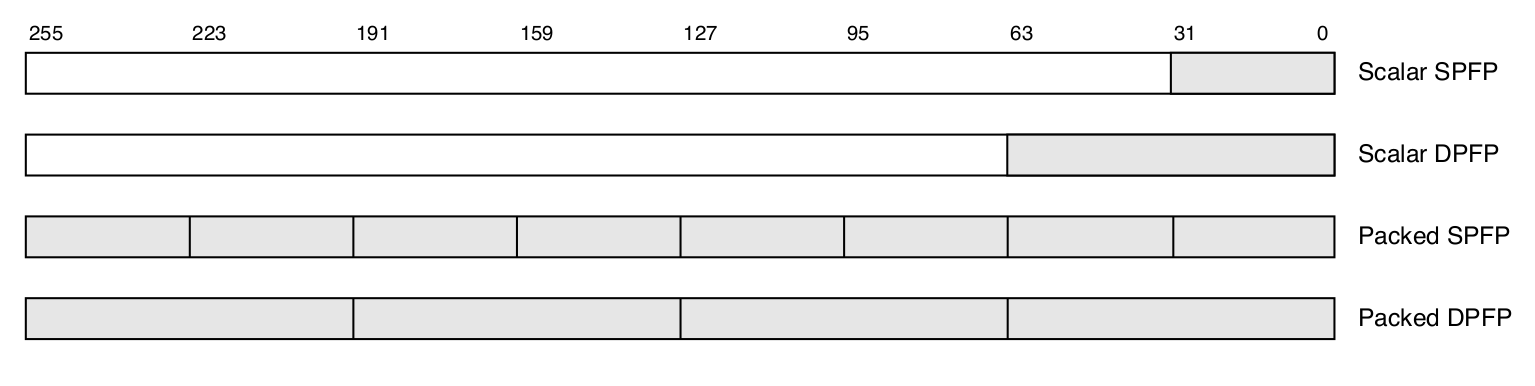
\includegraphics[width=\textwidth]{../images/Benz/avx_packed_scalar.png}
	\caption{Anordnung von Floats und Double in einem AVX SIMD Register} 
	\label{fig:avx_packed_scalar}
\end{figure}

Die Größe der Register wurde 1999 durch die Einführung von SSE, der Streaming SIMD Extension, verdoppelt. Der Namen der Register änderte sich zu \texttt{xmm0} bis \texttt{xmm7}. Die SSE erlaubte anfangs nur das packen von single precision floating points, was dem Datentyp Float entspricht. Die nächsten Jahre wurden mehrere Verbesserungen der SSE in neuere Generationen der CPUs verbaut, so unterstützten CPUs mit der SSE3 Hyper-Threading von SIMD Instruktionen.
2011 wurde AVX, Advanced Vector Extension, in der neuen Mikroarchitektur Sandy Bridge eingebaut. Diese fügte zu den Registern xmm0 bis mm7 die Register ymm0 bis ymm7 hinzu. Die Register können zu 8 großen Registern zusammengefasst werden, sodass die Registergröße für eine SIMD Operation 256 Bit beträgt. Auf CPUs mit 64 Bit Adressierung wächst die Anzahl der Register auf 16. 2013 wurde ein erweiterter Instruktionssatz, genannt AVX2, in die damals aktuelle Haswell Architektur eingebaut.
Die neuste Entwicklung im SIMD Umfeld nennt sich AVX-512. Dabei wird die Anzahl der Register nochmal verdoppelt auf 32 Register und es werden die neuen Register zmm0 bis zmm31 hinzugefügt. Diese haben eine Breite von 256 Bit. Werden die neuen Register mit den bereits aus der AVX vorhandenen Register zusammengefasst, erhöht sich die Datenbreite auf 512 Bit. Diese Version von AVX ist jedoch bis jetzt nur in sehr teuren CPUs, die für das Server Umfeld gedacht sind, enthalten (vgl. \cite{IntelAvx512}).
Ein Vergleich aller Register ist in der Grafik unterhalb zu erkennen.

\begin{figure}[!htbp]
	\centering
	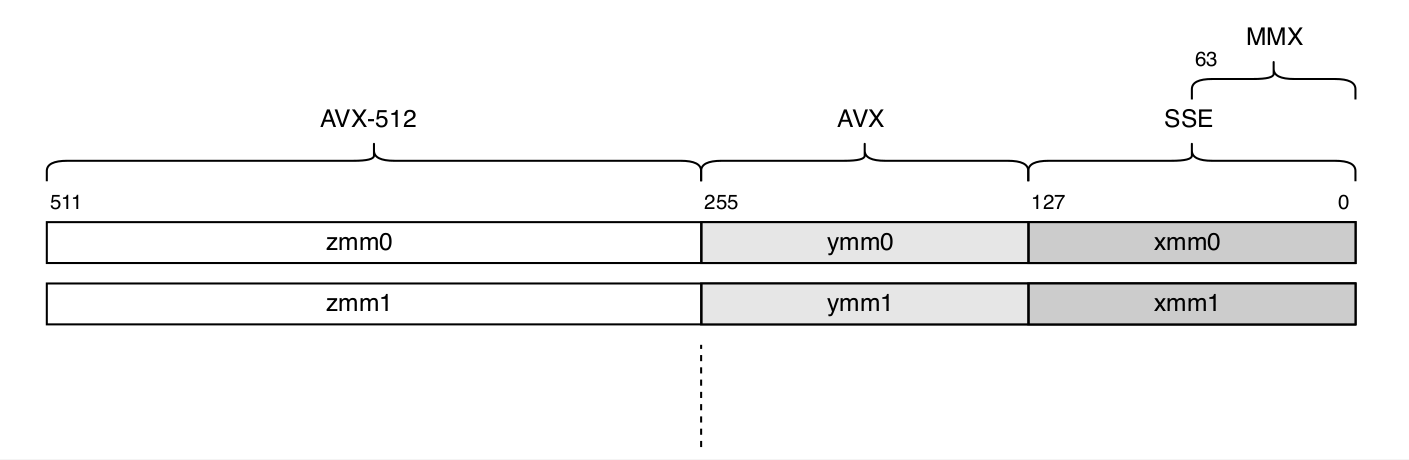
\includegraphics[width=\textwidth]{../images/Benz/simd_avx_sse_mmx.png}
	\caption{Übersicht der Größe von SIMD Registern der x86 Architektur} 
	\label{fig:simd_avx_sse_mmx}
\end{figure}

Eine für diese Arbeit interessante Funktion der SIMD Instruktionen von neuen x86 Architekturen ist die Multiplikation von Float Zahlen. Durch AVX-512 lassen sich bei einer neuen CPUs bis zu 16 Floats in einem Register unterbringen und mit einer Instruktion multiplizieren. Für die Multiplikation werden 2 Register benötigt, die mit den zu multiplizierenden Floats initialisiert sind. Desweiteren wird ein Register benötigt, in dem das Ergebnis gespeichert werden soll. Durch Aufrufen des Befehls zur Multiplikation werden das n-te Float in Register a mit dem n-ten Float in Register b multipliziert und in ein Zielregister geschrieben.
Da die neuste AVX-Version AVX-512 nur in wenigen CPUs integriert ist, wird in dieser Arbeit lediglich die ältere Version AVX2 verwendet.

\begin{figure}[!htbp]
	\centering
	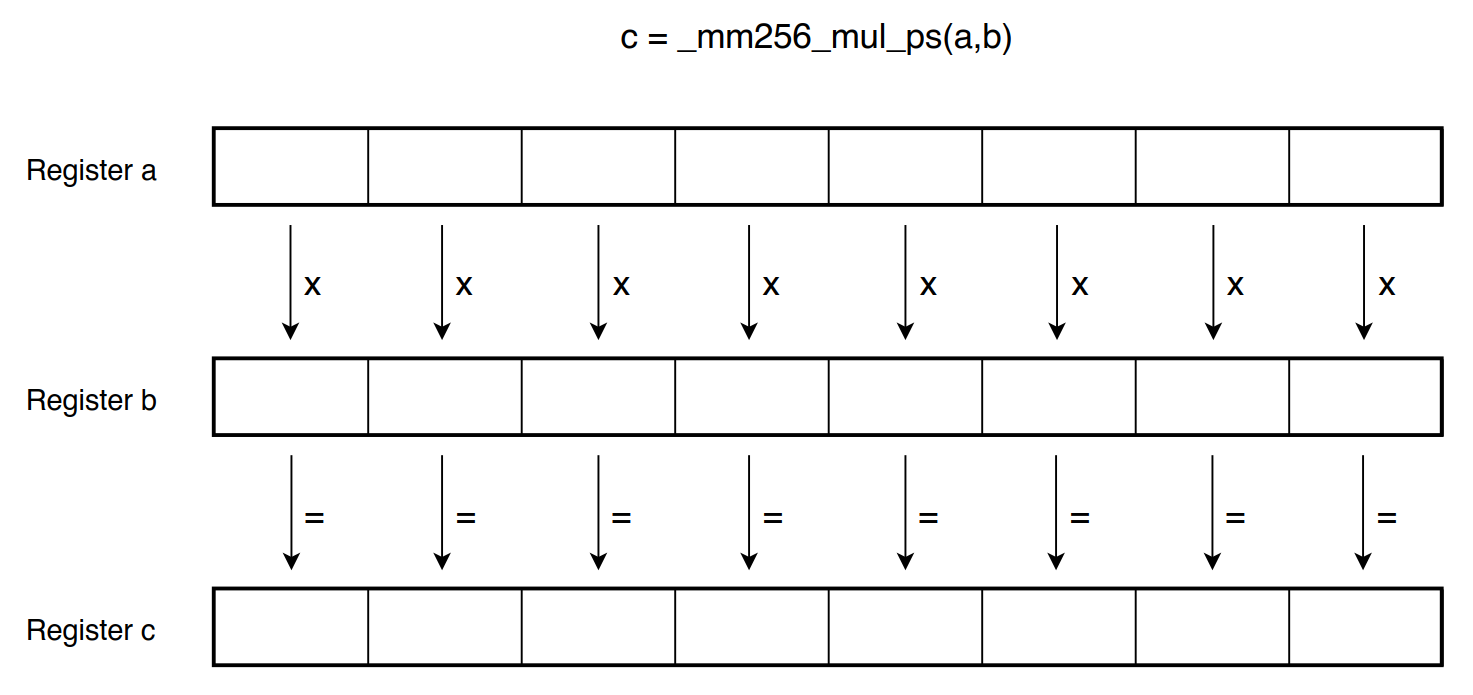
\includegraphics[width=\textwidth]{../images/Benz/avx.png}
	\caption{Multiplikation von 8 Floats durch eine SIMD Anweisung} 
	\label{fig:avx}
\end{figure}

In der Grafik werden 8 Multiplikationen von Floats mit der Instruktion \linebreak  \texttt{\_mm256\_mul\_ps()} gleichzeitig ausgeführt. Die \texttt{256} gibt hierbei an, wie groß die Register sind. In diesem Fall sind die Register 256 Bit groß. Anschließend wird die Rechenart angegeben, hier eine Multiplikation (\texttt{mul}). Das \texttt{p} steht hierbei für "packed". Alternativ kann ein \texttt{s} für "single slot" angegeben werden, dann wird lediglich an der hintersten Position ein Wert des Datentyps erwartet und für die Multiplikation verwendet. An letzter Stelle steht ein \texttt{s}. Dieses steht für "single precision", was dem Datentyp Float entspricht. Bei einem \texttt{d} an dieser Stelle wird "pouble precission", was dem Datentyp Double entspricht, angenommen.

Eine Übersicht aller SIMD-Instruktionen von Prozessoren mit aktueller x86-Architektur und findet sich unter \url{https://software.intel.com/sites/landingpage/IntrinsicsGuide}. Hier kann auch gesehen werden, mit welcher Erweiterung der SIMD Instruktionen ein Befehl einführt wurden ist.

Durch die Verwendung von AVX lässt sich die Zeit zum Multiplizieren von mehreren Floats, im Vergleich zur standardmäßigen Multiplikation, prinzipiell bis zu 16 mal verkürzen. Der gcc-Compiler versucht auf Optimierungsstufe 3 (Compilerflag \texttt{-O3}) for-Schleifen automatisch zu vektorisieren. Deswegen ist es nicht unbedingt vonnöten, die AVX-Register mühsam selbst zu verwenden. Durch das Compiler-Flag \texttt{-ftree-vectorizer-verbose=2} wird bei jeder Schleife ausgegeben, ob gcc den Code vektorisieren konnte und somit den Code mit SIMD-Instruktionen übersetzt hat oder nicht.

Die Instruktionen können jedoch auch explizit aufgerufen werden, sodass nicht der Compiler die Entscheidung übernimmt, wo und wie optimiert werden soll, sondern dies der Programmierer selbst Entscheiden kann. 

Für das Laden von Floats in ein AVX-Register gibt es mehrere Möglichkeiten. Um Werte an expliziter Stelle des Registers zu schreiben, gibt es den Befehl \texttt{\_mm256\_set\_ps(a8,a7,a6,a5,a4,a3,a2,a1)}. Der erste Parameter der Funktion wird hierbei an der letzten Stelle innerhalb des Registers geschrieben. Um einen Wert an alle Stellen des Registers zu schreiben, kann \texttt{\_mm256\_set1\_ps(a1)} verwendet werden. Mit \texttt{\_mm256\_load\_ps(addr)} kann eine Adresse übergeben werden und die folgenden Werte an dieser Adresse werden in das Register geschrieben. 
Um das Ergebnis wieder als Floats anzusprechen, muss der Pointer zum Ergebnisregister als Pointer zu einem Float-Array gecastet werden.

\begin{lstlisting}[language=c++, caption=Multiplikation mit AVX, captionpos=b, label=listing:avx_multiplikation, frame=single, linewidth=\textwidth, breaklines=true]
float array[8]=[1,2,3,4,5,6,7,8];
_m256 a = _mm256_set_ps(8,7,6,5,4,3,2,1);
_m256 b = _mm256_load_ps(array);
_m256 res = _mm256_mul_ps(a,b);
float *f = (float*)&res;
\end{lstlisting}
An Adresse \texttt{f} stehen nun die ersten 8 Quadratzahlen, die alle mit der Instruktion \texttt{\_mm256\_mul\_ps} auf einmal errechnet wurden.


\section{Implementierung des Convolutional Neural Network}

Zur Implementierung des Convolutional Neural Networks auf einer x86-Architektur wurde die serielle Implementierung als Grundlage verwendet. Diese wurde genauer in Kapitel \nameref{chap:seriell} beschrieben. Zur optimierten Ausführung auf einer x86-CPU muss das Programm umgeschrieben werden. Folgende Methoden wurden zur Optimierung verwendet:
\begin{itemize}
	\item Reduzierung der Schreibzugriffe
	\item Reduzierung der zufälligen Lesezugriffe
	\item Cache-Hierarchie ausnutzen
	\item SIMD-Architektur ausnutzen
\end{itemize}

\subsection{Die Klasse Tensor}
Für jegliche Inputs und Outputs aller Layer wurde die Klasse \texttt{Tensor} erstellt. Diese beinhaltet ein Array aus Floats sowie drei Integer mit den Namen \texttt{x}, \texttt{y} und \texttt{z}. \par 
Im Konstruktor werden die Werte von \texttt{x}, \texttt{y} und \texttt{z} übergeben. Es gibt auch Konstruktoren mit nur 2 oder nur 1 Parameter, die anderen Dimensionen werden dann aus 1 gesetzt. Die Tensor-Klasse kann somit auch Matritzen oder Vektoren abbilden. \par 
Das Array hat als Länge das Produkt aus allen 3 Dimensionen. Die Reihenfolge ist hierbei so angeordnet, wie die Leserichtung eines Buches. Es wird immer eine Zeile durchgegangen, bevor die nächste Zeile im Speicher liegt. Ist die letzte Zeile einer Seite erreicht, liegt die erste Zeile der nächsten Seite im Speicher bis der Tensor vollständig im Speicher abgebildet ist. \par
Die Tensor-Klasse bietet Funktionen, um die Adresse des Arrays an bestimmten Stellen zu finden. Dabei wird zuerst die z-Position und Anschließend die y-Position angegeben.
\begin{lstlisting}[language=c++, caption=Funktion zum Erhalten eines Pointers auf den Tensor, captionpos=b, label=listing:tensor_get_array, frame=single, linewidth=\textwidth, breaklines=true]
float *Tensor::getArray(int z, int y){
	assert(z<this->z);
	assert(y<this->y);
	return array+z*this->y*x+y*x;
}
\end{lstlisting}
Die x-Position kann bei dieser Funktion nicht angegeben werden. Um die genaue Adresse zu erhalten, muss ein Offset in Höhe der x-Position angegeben werden. Danach zeigt der Zeiger auf die gewünschte Stelle. Durch die Verwendung eines Zeigers, kann die Funktion sowohl zum Lesen als auch zum Schreiben an dieser Position verwendet werden.
\begin{lstlisting}[language=c++, caption=Verwendung der getArray()-Funktion, captionpos=b, label=listing:verwendung_get_array, frame=single, linewidth=\textwidth, breaklines=true]
zeiger = tensor->getArray(z_pos, y_pos)[x_pos];
\end{lstlisting}
Die Klasse besitzt noch Funktionen, um die Größe des Tensors in die drei verschiedenen Dimensionen auszugeben. Dadurch kann mit drei verschachtelten For-Schleifen einfach durch alle Elemente iteriert werden.

\subsection{die verschiedenen Layertypen}
Es gibt drei verschiedene Layertypen. Diese sind der Convolutional Layer, der Max Pooling Layer und der Fully Connected Layer. Um diese drei verschiedenen Layer in einer gemeinsamen Liste zu speichern, wurde ein Union mit dem Namen \texttt{Layer} erstellt. Dieses Union kann einen dieser 3 Datentypen annehmen. 
Jede dieser Layer besitzt mehrere Zeiger auf Tensoren. Jeder Layer hat Zeiger auf Tensoren die die Activation, den Output und den Gradienten des Layers und des Layers davor darstellen. Mit Ausnahme des Max Pooling Layers gibt es noch Zeiger auf Gewichte und Biases, sowie Tensoren mit den Deltas der Gewichte und Biases. Der Zeiger auf den Output eines Layers hat den selben Wert wie der Zeiger des Inputs des folgenden Layers. Somit weden die Tensoren von mehreren Layern verwendet, einmal als Input und einmal als Output. Das Gleiche gilt für die Gradienten. Die Tensoren sind so aufgebaut, dass die x und y Dimension ein Muster darstellt und mit der z-Position die verschiedenen Muster ausgewählt werden.
Alle Layer beinhalten die Methoden \texttt{generate()}, \texttt{forward()}, \texttt{backward()} und \texttt{fix\_weights()}.
 Die \texttt{generate()} Methode benötigt als Parameter Zeiger zu den Tensoren der Activation und der Gradienten der Activation des Layers. Diese sind, ausgenommen des ersten Layers in einem Netzwerk, die Outputs der vorherigen Layer. Die \texttt{generate()} Methode berechnet aufgrund der Parameter der Methode und der Parameter des Konstruktors des Layers die Größen alles Tensoren die vom Layer verwendet werden.
Die Funktionen \texttt{forward()} und \texttt{backward()} nehmen keine Parameter an. Erstere wird aufgerufen, um die Inputs der Neuronen durch das Netzwerk zu propagieren. Letztere wird aufgerufen, um die Fehler zurück zu propagieren. 
Bevor die \texttt{backward()} Methode aufgerufen werden kann, muss der Fehler im letzten Layer berechnet werden und in den Tensor der Gradienten gespeichert werden. Die Formel für die Berechnung des Fehlers, bei Verwendung von Quadratic Coast als Kostenfunktion, ist in \ref{eq:fehler_in_letztem_layer} zu sehen.
\begin{equation}\label{eq:fehler_in_letztem_layer}
\begin{split}
\frac{\partial C}{\partial a_j^L} = ( a_j^L - y_j )
\end{split}
\end{equation}
$a_j^L$ ist hierbei ein Output im Letzten Layer und $y_j$ das dazu gehörende gewünschte Ergebnis. Auf die partielle Ableitung der Kostenfunktionen nach dem Output wird anschließend noch die inversen Sigmoid-Funktion angewandt.

Durch die Funktion \texttt{fix\_weights()} werden die Deltas benutzt, um die Gewichte und die Biases anzupassen. Dabei wird die Batch-Größe angegeben sowie die Trainingsrate. Nach Aufruf dieser Funktion werden alle Deltas auf 0 gesetzt. Dadurch kann eine Batch von Inputs verwendet werden, da die Funktion \texttt{backward()} die Deltas von Biases und Gewichten auf den bestehenden Wert addiert.

\begin{figure}[!htbp]
	\centering
	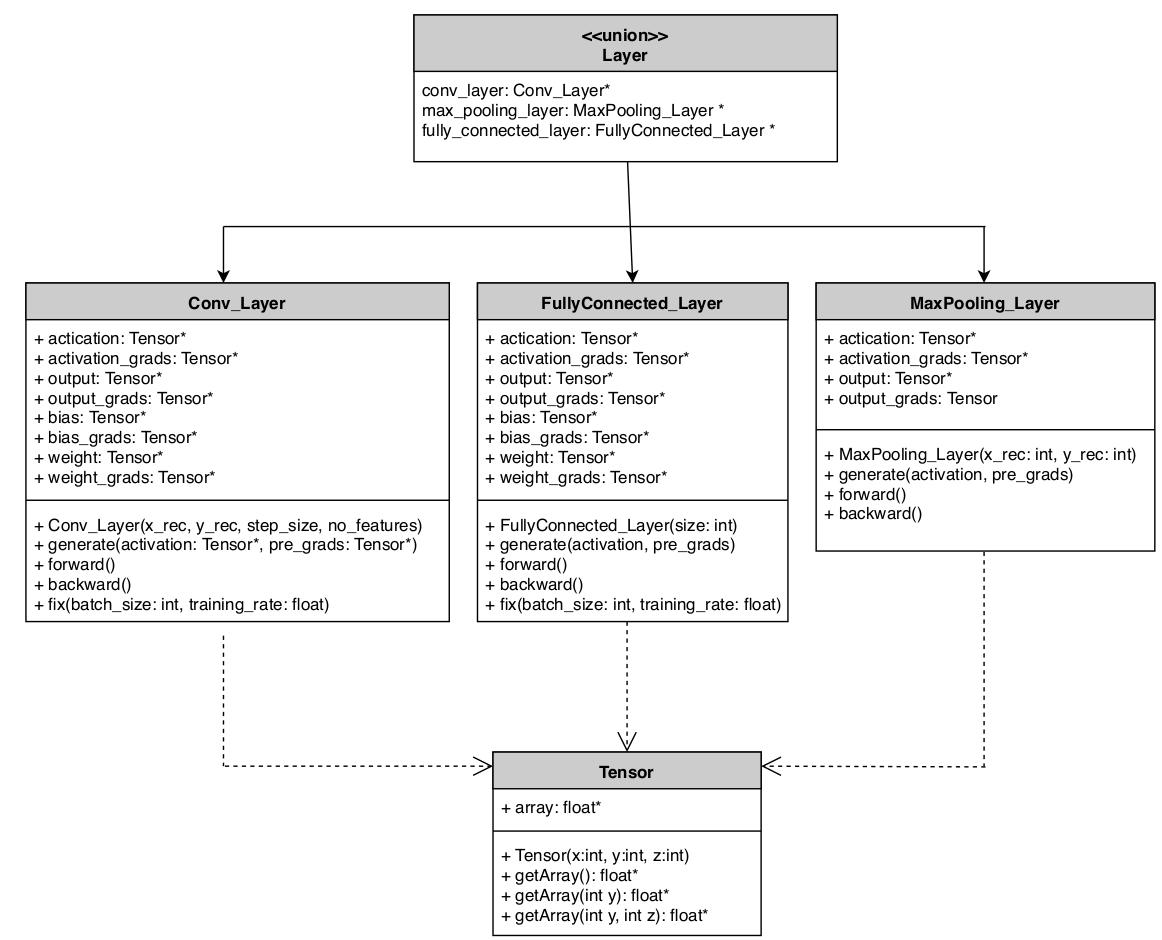
\includegraphics[width=\textwidth]{../images/Benz/UML_Layer.png}
	\caption{UML-Diagramm der Layer} 
	\label{fig:uml_layer}
\end{figure}

Ein Max Pooling Layer erwartet als Parameter im Konstruktor die Schrittweite, in dem das Max Pooling stattfinden soll. Die Größe des Outputs ist der Quotient der Dimensionen des Inputs dividiert durch die Schrittweite in dieser Dimension. Die z-Dimensionen des Inputs und des Outputs sind die selben. Dasselbe gilt für die Gradienten. In der \texttt{forward()} Methode wird immer das Maximum im gewünschten Bereich gesucht und anschließend in den Output geschrieben. Die \texttt{backward} Methode leitet den Gradienten des Layers danach an die Position, die den maximalen Bereich in diesem Bereicht hatte, weiter. Die Klasse hat den Namen \texttt{MaxPoolingLayer}

Die Klasse \texttt{FullyConnectedLayer} erwartet im Konstruktor die Anzahl der Neuronen in diesem Layer. Der Output ist ein Vektor mit dieser Anzahl an Elementen. Der Vektor wird als Tensor mit allen Dimensionen, außer der x-Dimension, auf 1 abgebildet. Als Gewichts-Tensor wird die Dimension der Activation verwendet, die x-Dimension wird jedoch mit der Neuronenanzahl des Layers multipliziert. Die Gewichte für einen Output sind damit sehr einfach zu finden und es kann sich ein beliebiger Layer vor dem Fully Connected Layer befinden, ohne den Code für die verschiedenen Layertypen zu ändern. Der Bias-Tensor hat die gleiche Dimension wie der Output-Tensor.

\texttt{ConvLayer} ist der Klassennamen für den Convolutional Layer. Im Constructor wird die Größe der Faltungskerne, die Anzahl der zu ermittelnten Features und die Schrittweise zum Abfahren der Activation angegeben. Die Größe des Outputs lässt sich mit dieser Formel berechnen.
\begin{equation}\label{eq:cnn_outout_size}
\begin{split}
size_{output} = \frac{size_{input} -size_{faltungskern} +1}{schrittweite}
\end{split}
\end{equation}
Die z-Dimension des Outputs ist durch die Anzahl der Features gegeben. Der Tensor der Gewichte, im Convolutional Layer der Faltungskerne, entspricht in x- und y-Richtung der übergebenen Größe der Faltungskerne. Die Größe in z-Richtung entspricht dem Produkt aus der z-Dimension der Activation und der Summe an Features. Für jedes Feature ist so ein Teilstück des Gewichtstensors vorhanden. Für jedes Feature gibt es einen Eintrag in einem Tensor mit einer Dimension als Bias.

Die Klasse \texttt{InputLayer}, die es noch in der seriellen Implementierung gab, gibt es nicht mehr. Stattdessen zeigt der Pointer des ersten Layers auf einen Tensor, der direkt das Bild enthält, welches im Netzwerk analysiert werden soll.

\subsection{Funktion der verschiedenen Tensoren}
Die Grafik \ref{fig:conv_forward_backward} zeigt das Zusammenspiel und die Funktionsweise der verschiedenen Tensors bei Verwendung der forward()- und backward()-Funktionen. Die Abkürzung "w" steht hierbei für "weight", "b" für "bias", "w\_g" für "weight\_grads" und "b\_g" für "bias\_grads". In einem Layer sind immer Zeiger zu den Gewichten und den Biases, die sich in der Grafik vor dem Layer befinden, enthalten. In forward-Richtung werden die Gewichts- und die Bias-Tensors für die Berechnung der Activation des nächsten Layers verwendet. Im letzten Layer wird der Fehler berechnet und in den Tensor "output\_grad" geschrieben. In backward-Richtung werden nun die Fehler zurückgerechnet und dabei in jedem Layer die Tensoren "weight\_grads" und "bias\_grads" geschrieben. Die Werte für die Tensoren werden auf den sich schon darin befindenden Wert addiert.
Durch Aufruf der fix()-Funktion werden die Gewichte und Biases der Layer durch die Werte Tensoren "weight\_grads" und "bias\_grads" angepasst. Dies ist in der Grafik als orangefarbenen Pfeil zu erkennen.
\begin{figure}[!htbp]
	\centering
	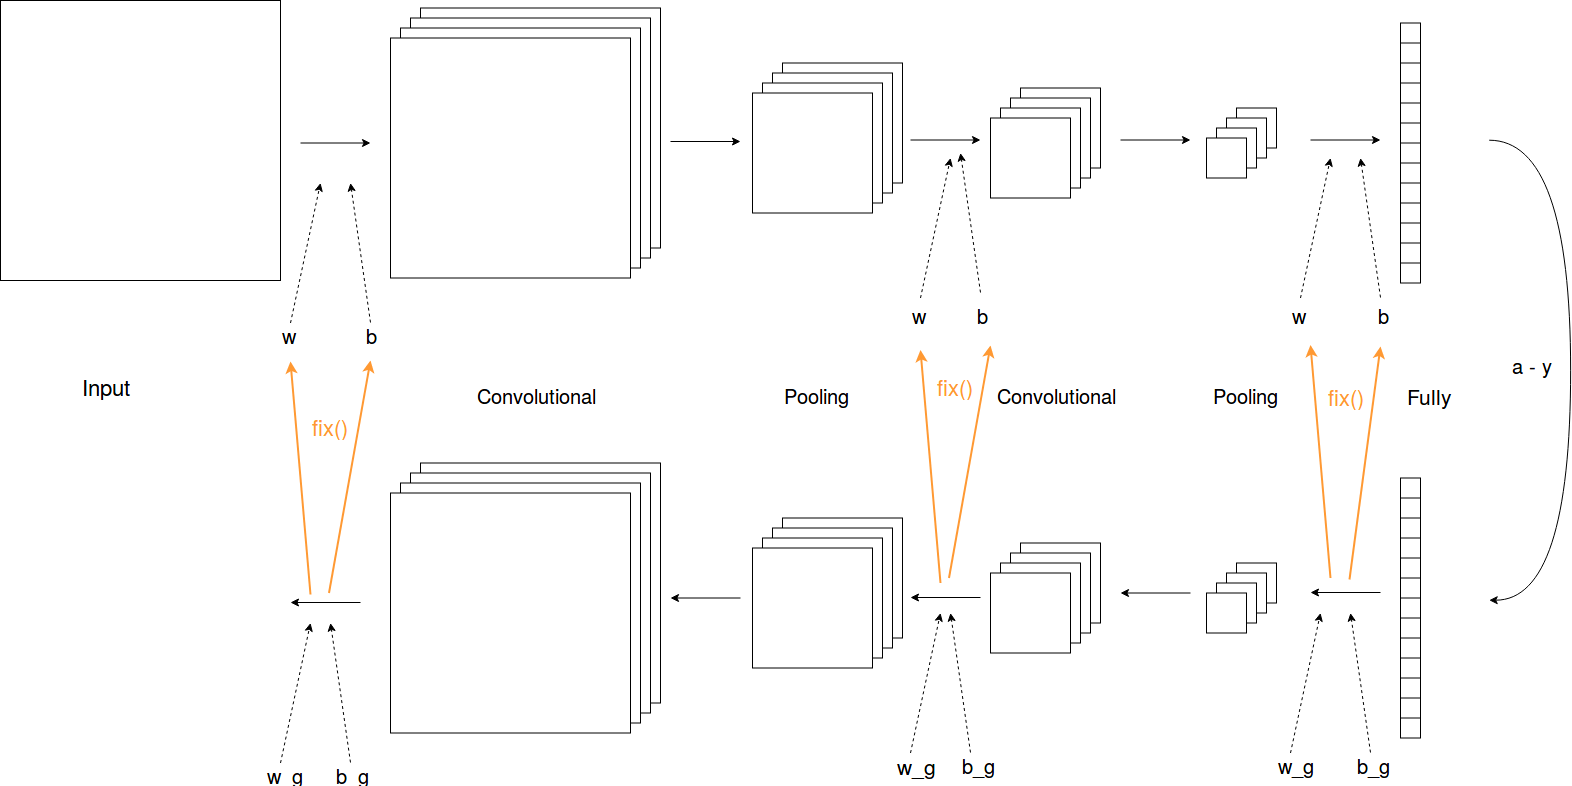
\includegraphics[width=\textwidth]{../images/Benz/forward_backward.png} %Grafik Forward Backward
	\caption{Zusammenspiel zwischen forward()- und backward()-Methode} 
	\label{fig:conv_forward_backward}
\end{figure}

\subsection{Implementierung des Convolutional Layers}

Die größten Optimierungsmöglichkeiten ergeben sich im Convolutional Layer, da dort die Anzahl der Multiplikationen am Höchsten ist. Um den Layer zu optimieren, muss zuerst die Funktionsweise aus der seriellen Implementierung analysiert werden.

Bei der seriellen Implementierung werden die benötigten Elemente der Activation für eine Faltungsoperation in einen temporären Vektor geschrieben. Dieser Vektor wird anschließend mit einer Gewichts-Matrix multipliziert. Dies stellt die Faltung mit allen Kernen für diese Elemente der Activation dar. Das Ergebnis der Multiplikation wird wiederum in einen anderen temporären Vektor gespeichert, zu welchem ein Bias Vektor elementweise addiert wird. Das Ergebnis sind die Elemente des Outputs an einer Stelle in allen Features. Die Vorgehensweise ist in der Grafik unterhalb zu sehen.

\begin{figure}[!htbp]
	\centering
	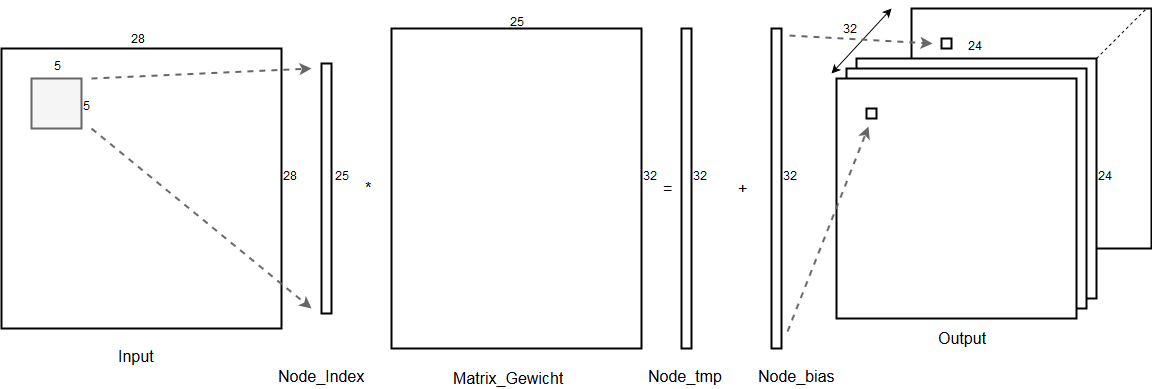
\includegraphics[width=\textwidth]{../images/Benz/Conv_Layer_Seriel.png} %Grafik Ablauf Convolutional Layer Seriell
	\caption{Ablauf des Convolutional Layers in der seriellen Implementierung} 
	\label{fig:conv_layer_seriell}
\end{figure}


Bei dieser Vorgehensweise sind sehr viele neue Allokationen des Hauptspeichers nötig, da viel Speicherplatz kurzfristig benötigt wird. Dies lässt sich vermeiden, indem die Multiplikationen geschickt nacheinander ausführt und das Ergebnis direkt an die Zieladresse geschrieben werden. 

\subsubsection{Durchgehen der Activation}

Es wurde sich für eine Methode entschieden, bei der zuerst der Output-Tensor auf 0 gesetzt wird. Anschließend wird jedes Element vom Activation-Tensor durchgegangen. Je nachdem, wo sich das Element im Activation-Tensor befindet, gibt es verschiedene Elemente der Gewichts-Matritzen, mit denen es multipliziert werden muss. Beispielweise muss das erste Element links oben nur mit dem Element links oben des Faltungskerns multipliziert werden, währenddessen Elemente in der Mitte des Input-Tensors mit allen Elementen des Faltungskerns multipliziert werden müssen. Die Ergebnisse müssen je nach Element des Faltungskerns an verschiedenen Stellen im Output geschrieben werden.
Die entsprechenden Elemente des Faltungkerns werden mit zwei if-Bedingungen ermittelt. Bei diesen if-Bedingungen wird der Start- und der Endindex für beide Dimensionen eines Faltungskerns durch die Position des Elements in der Activation ermittelt. Anschließend werden diese Werte des Faltungskerns mit dem einen Element des Inputs multipliziert und die Ergebnisse an die richtige Stelle des Output-Tensors hinzugefügt.

In unten stehender Formel ist der Vorgang zu erkennen. x\_pos und y\_pos sind die Indizes des Faltungskerns mit dem das Element \(a_{x,y,z}\) multipliziert werden muss. Alle Kombinationen von x\_pos, y\_pos und z\_pos werden durchgegangen. Anschließend wird das nächste Element von \(a\) verwendet.
\begin{equation}
\begin{split}
x\_pos = {min\_x_{a_{x,y,z}}\ ..\ max\_x_{a_{x,y,z}}}\\
y\_pos = {min\_y_{a_{x,y,z}}\ ..\ max\_y_{a_{x,y,z}}}\\
z\_pos = {z\ ..\ length(w_{z})\ [SW:\ length(a_{z})]}\\
o_{x-x\_pos,y-y\_pos,z\_pos/z} += a_{x,y,z}*w_{x\_pos,y\_pos,z\_pos}
\end{split}
\end{equation}
Den Programmcode ist in \ref{listing:conv_activation} zu sehen.

\begin{lstlisting}[language=c++, caption=Convolution: Activation durchgehen, captionpos=b, label=listing:conv_activation, frame=single, linewidth=\textwidth, breaklines=true]
#pragma omp for firstprivate(output, activation, weight) lastprivate(output, activation, weight)
for(int pre_z_pos=0; pre_z_pos < activation->getZ(); pre_z_pos++){
   for(int pre_y_pos = 0; pre_y_pos < activation->getY(); pre_y_pos++){
      for(int pre_x_pos = 0; pre_x_pos < activation->getX();pre_x_pos++){

         int start_x_rec=0;
         int stop_x_rec=x_receptive-1;
         if(pre_x_pos < x_receptive-1) stop_x_rec = pre_x_pos;
         else if(pre_x_pos > activation->getX()-x_receptive) start_x_rec = x_receptive + pre_x_pos - activation->getX();

         int start_y_rec=0;
         int stop_y_rec=y_receptive-1;
         if(pre_y_pos < y_receptive-1) stop_y_rec = pre_y_pos;
         else if(pre_y_pos > activation->getY()-y_receptive) start_y_rec = y_receptive + pre_y_pos - activ[language=c++]ation->getY();
         
         for(int z_pos=pre_z_pos;z_pos < weight->getZ();z_pos+=activation->getZ()){
            for(int y_rec = start_y_rec; y_rec <= stop_y_rec ; y_rec++){
               for(int x_rec = start_x_rec; x_rec <= stop_x_rec ; x_rec++){
                  output->getArray(z_pos/activation->getZ(), pre_y_pos-y_rec)[pre_x_pos-x_rec] += activation->getArray(pre_z_pos,pre_y_pos)[pre_x_pos] * weight->getArray(z_pos,y_rec)[x_rec];
               }
            }
         }
      }
   }
}
\end{lstlisting}

Durch diese Methode kann der Output-Tensor und die Gewichte im Cache liegen, die Speicherzugriffe erfolgen somit sehr schnell. Da kein neuer Speicher allokiert wird, muss nicht darauf gewartet werden, bis der vergleichsweise sehr langsame Arbeitsspeicher den Speicherplatz freigibt und die Daten in den Cache geladen werden können. 

\subsubsection{Durchgehen des Outputs}

Der Convolutional Layer kann auf mehrere Arten implementiert werden. Immer müssen mehrere For-Schleifen ineinander die Faltung mit dem Faltungskern ausführen, dazu werden die einzelnen Zählvariablen als Index des Input und des Outputs verwendet. Es kann jedoch entschieden werden, welche Schleife für welchen Indes verwendet wird.

Die wohl einfachste Art der Implementierung ist die, dass die äußeren For-Schleifen den Index des Outputs bestimmen und die inneren den Index des Inputs und des Faltungskerns. Bei dieser Art kann der Index des Outputs als Anfangsindex des Inputs verwendet werden. Dies kann anhand der Formel für die Größe des Outputs in Abhängigkeit des Inputs und der Größe des Faltungskerns hergeleitet werden. Die inneren Schleifen erzeugen einen Offset zwischen 0 und der Breite/Länge des Faltungskerns. Dieser Offset wird auf die Variable des Outputs addiert und erzeugt somit die Positionen des Inputs, die für den Output verwendet werden soll.

Eine Implementierung des Convolutional Layers nach dieser Methode ist unterhalb zu erkennen.
\begin{lstlisting}[language=c++, caption=Convolution: Output durchgehen, captionpos=b, label=listing:conv_output, frame=single, linewidth=\textwidth, breaklines=true]

#pragma omp parallel for firstprivate(output, activation, weight) lastprivate(output, activation, weight)
for ( int z_pos =0; z_pos < output->getZ() ; z_pos++){
   for ( int y_pos = 0 ; y_pos < output->getY() ; y_pos++){
      for ( int x_pos = 0 ; x_pos < output->getX() ; x_pos++){
         
         int z_stop = (z_pos+1)*activation->getZ();
         for ( int w_z_pos=z_pos*activation->getZ() ; w_z_pos < z_stop; w_z_pos++){
            for ( int w_y_pos = 0; w_y_pos < weight->getY (); w_y_pos++){
               for ( int w_x_pos = 0 ; w_x_pos < weight->getX(); w_x_pos++){
                  output->getArray(z_pos, y_pos)[x_pos] += activation->getArray(z_pos%activation->getZ(), y_pos+w_y_pos)[x_pos+w_x_pos] * weight->getArray(w_z_pos, w_y_pos )[w_x_pos] ;
               }
            }
         }
      
      }
   }
}
\end{lstlisting}

Der Vorteil dieser Methode, im Vergleich zur vorherigen Methode, ist die einfache Umsetzung von SIMD Instruktionen in diesem Code. Werden AVX-Register verwendet, können immer 8 der Gewichte in ein mmx-Register geladen werden. In ein zweites Register müssen die Werte der Activation geladen werden. Anschließend können die erhaltenen Ergebnisse zusammenaddiert werden. Dies wird solange wiederholt, bis alle Multiplikationen für einen Output des Layers abgeschlossen sind.
Ein weiterer Vorteil ist die Tatsache, dass die Sigmoid-Funktion direkt innerhalb der Schleife angewandt werden kann. Bei der Implementierung, in der die Activation in der äußeren Schleife durchgegangen wird, muss die Sigmoid-Funktion in einer separaten Schleife auf alle Outputs angewandt werden.

Für die explizite Verwendung der AVX-Register wurde dieser Code entwickelt, der innerhalb der äußeren drei Schleifen eingesetzt werden muss. Es werden immer acht Multiplikationen für einen Output gleichzeitig ausgeführt. Ist Anzahl der Multiplikationen nicht durch 8 teilbar, werden mit der letzten SIMD-Anweisung weniger Multiplikationen ausgeführt. Alle Ergebnisse für einen Faltungskern werden zusammenaddiert und in den Output geschrieben.

\begin{lstlisting}[language=c++, caption=Implementierung des Convolutional Layers mit AVX, captionpos=b, label=listing:conv_avx, frame=single, linewidth=\textwidth, breaklines=true]
int z_stop = (z_pos+1)*activation->getZ();

float array [8];

for(int w_z_pos = z_pos*activation->getZ(); w_z_pos < z_stop; w_z_pos++){

mmx1 =  _mm256_loadu_ps(weight->getArray(w_z_pos));
int mmx_index = 0;

for(int w_y_pos = 0; w_y_pos < weight->getY(); w_y_pos++){
   for(int w_x_pos = 0; w_x_pos < weight->getX(); w_x_pos++){
   
      array[mmx_index%8]=activation->getArray(w_z_pos%activation->getZ(), y_pos+w_y_pos)[x_pos+w_x_pos];
      mmx_index++;
      if(mmx_index%8 == 7 || mmx_index == weight->getSize()-1){
         mmx2 = _mm256_loadu_ps(array);
         mmxres = _mm256_mul_ps(mmx1, mmx2);
         float *f = (float*)&mmxres;
         for(int i=0; i < 8 && mmx_index+i < weight->getSize(); i++){
            output->getArray(z_pos,y_pos)[x_pos] += f[i];
         }
         mmx1 =  _mm256_loadu_ps(weight->getArray(w_z_pos)+mmx_index);
      }
      
   }
}
\end{lstlisting}

\subsubsection{Vergleich der verschiedenen Implementierungen}

Die verschiedenen Implementierungen des Convolutional Layers wurden in einem Testprogramm auf ihre Laufzeiten analysiert. Dabei wurde eine Activation mit der Größe von 24*24*32 gewählt und ein Output von 20*20*64. Die Faltungskerne haben jeweils 25 Elemente, es wird immer eine 5*5-Umgebung nach Mustern abgesucht.
Als Testhardware wurde ein PC mit einer Intel Core i5-5310 CPU verwendet. Diese besitzt lediglich 2 CPU Kerne.
In einem Durchlauf des Programms werden 10 Faltungsoperationen mit jeder der drei Implementierungen ausgeführt. Die Implementierungen sind einmal das Durchgehen des Outputs mit AVX, einmal das Durchgehen des Outputs ohne AVX und die Implementierung, bei der der Input durchgegangen wird. Die Ausführungszeiten werden in Sekunden gemessen. 
Als Optimierungsstufe wurde die Optimierungsstufe 0 und die Optimierungsstufe 3 im Compiler gcc verwendet. Dies einmal mit, und einmal ohne Verwendung von OpenMP.
Gemessen wurde mit der Funktion \texttt{clock()}. Diese Funktion gibt eine Zahl zurück, die sich bei  jedem Tick auf dem Prozessor erhöht. Durch die Differenz der Zahlen vor- und nach der Ausführung eines Codes, lässt sich die Anzahl der Ticks zur Ausführung des Codes ermitteln. Die gemessene Differenz wurde durch eine Million geteilt um kleinere Zahlen zu erhalten.

\begin{tabular}{|p{3.5cm}|p{3cm}|p{3cm}|p{3cm}|}
\hline
Optimierungsstufe & Output AVX & Output & Input \\
\hline
O0 & 10,27 \linebreak 13,26 \linebreak 7,63 & 7,79 \linebreak 11,44 \linebreak 5,6 & 8,51 \linebreak 11,45 \linebreak 6,13 \\
\hline
O3 & 4,44 \linebreak 4,22 \linebreak 4,87 & 3,64 \linebreak 3,32 \linebreak 4,3 & 3,49 \linebreak 3,15 \linebreak 3,82 \\
\hline
O0, OpemMP & 9,95 \linebreak 10,29 \linebreak 9,2 & 7,38 \linebreak 8,29 \linebreak 7,04 & 7,85 \linebreak 8,15 \linebreak 7,6 \\
\hline
O3, OpenMP & 4,77 \linebreak 4,31 \linebreak 5,73 & 4,1 \linebreak 3,52 \linebreak 4,98 & 4,22 \linebreak 3,73 \linebreak 5,332 \\
\hline
\end{tabular}

Da die Laufzeiten teilweise sehr unterschiedlich ausfallen, wurden drei Durchläufe des Programms pro Optimierungsstufe getätigt.
Es ist zu erkennen, dass die Verwendung von OpenMP aus Optimierungsstufe 0 nur zu einer sehr kleinen Geschwindigkeitsverbesserung führt. Auf Optimierungsstufe 3 verschlechtert sich das Ergebnis durch parallele Ausführung sogar. Dies liegt klar an der CPU der Testhardware, die lediglich 2 Kerne besitzt. Das Erstellen von neuen Threads ist zu aufwändig im Vergleich zum erhaltenen Performance-Gewinn. Um einen Leistungsgewinn durch Multithreading zu erzielen, muss die CPU mehrere Kerne besitzen oder das Programm besser parallelisiert werden. 
Eine weitere, interessante Erkenntnis aus diesem Vergleich ist, dass die Implementierung mit expliziten AVX-Aufrufen langsamer ist als die Implementierung ohne AVX. Der Compiler schafft es, den Code besser zu optimieren als mein Versuch, die Intrinsiks zu verwenden. Die Implementierung, bei der der Input durchgegangen wird auf Optimierungsstufe 3, ist die schnellste Implementierung. Dies liegt höchstwahrscheinlich an der Ausnutzung der Cache-Hierarchie. Der Input kann bei dieser Implementierung immer im Speicher gelassen werden und wird eins nach dem anderen Durchgegangen.

Den Code tatsächlich zu optimieren, wurde im Rahmen der Studienarbeit nicht geschafft. Für das Suchen eines Fehlers beim Zurückrechnen der Biases und Gewichte wurde zu viel Zeit investiert. Die Zeit für das tatsächliche Optimieren mit SIMD und Multithreading viel deswegen zu gering aus, um den Zeitrahmen der Studienarbeit nicht komplett zu sprengen.
Trotzdem wurden Messungen mit dem Programm ausgeführt, die im letzten Kapitel dieser Arbeit, Kapitel \ref{chap:vergleich}, beschrieben sind.

\end{document}